ATLAS (a not terribly natural acronym for ``A Toroidal LHC Apparatus'') is a general purpose detector designed to maximize the detection efficiency of all physics objects, including leptons, jets, and photons. This means it is capable of measuring all (sufficiently long-lived) SM particles, with the exception of neutrinos, the presence of which can be inferred based on missing transverse momentum. The detector measures 44 m long, and 25 m tall. 

The ATLAS detector consists of multiple concentric layers, each of which serves a different purpose in reconstructing collisions. At the very center of the detector is the interaction point where the proton beams of the LHC collide. 

\begin{figure}[H]
\centering
   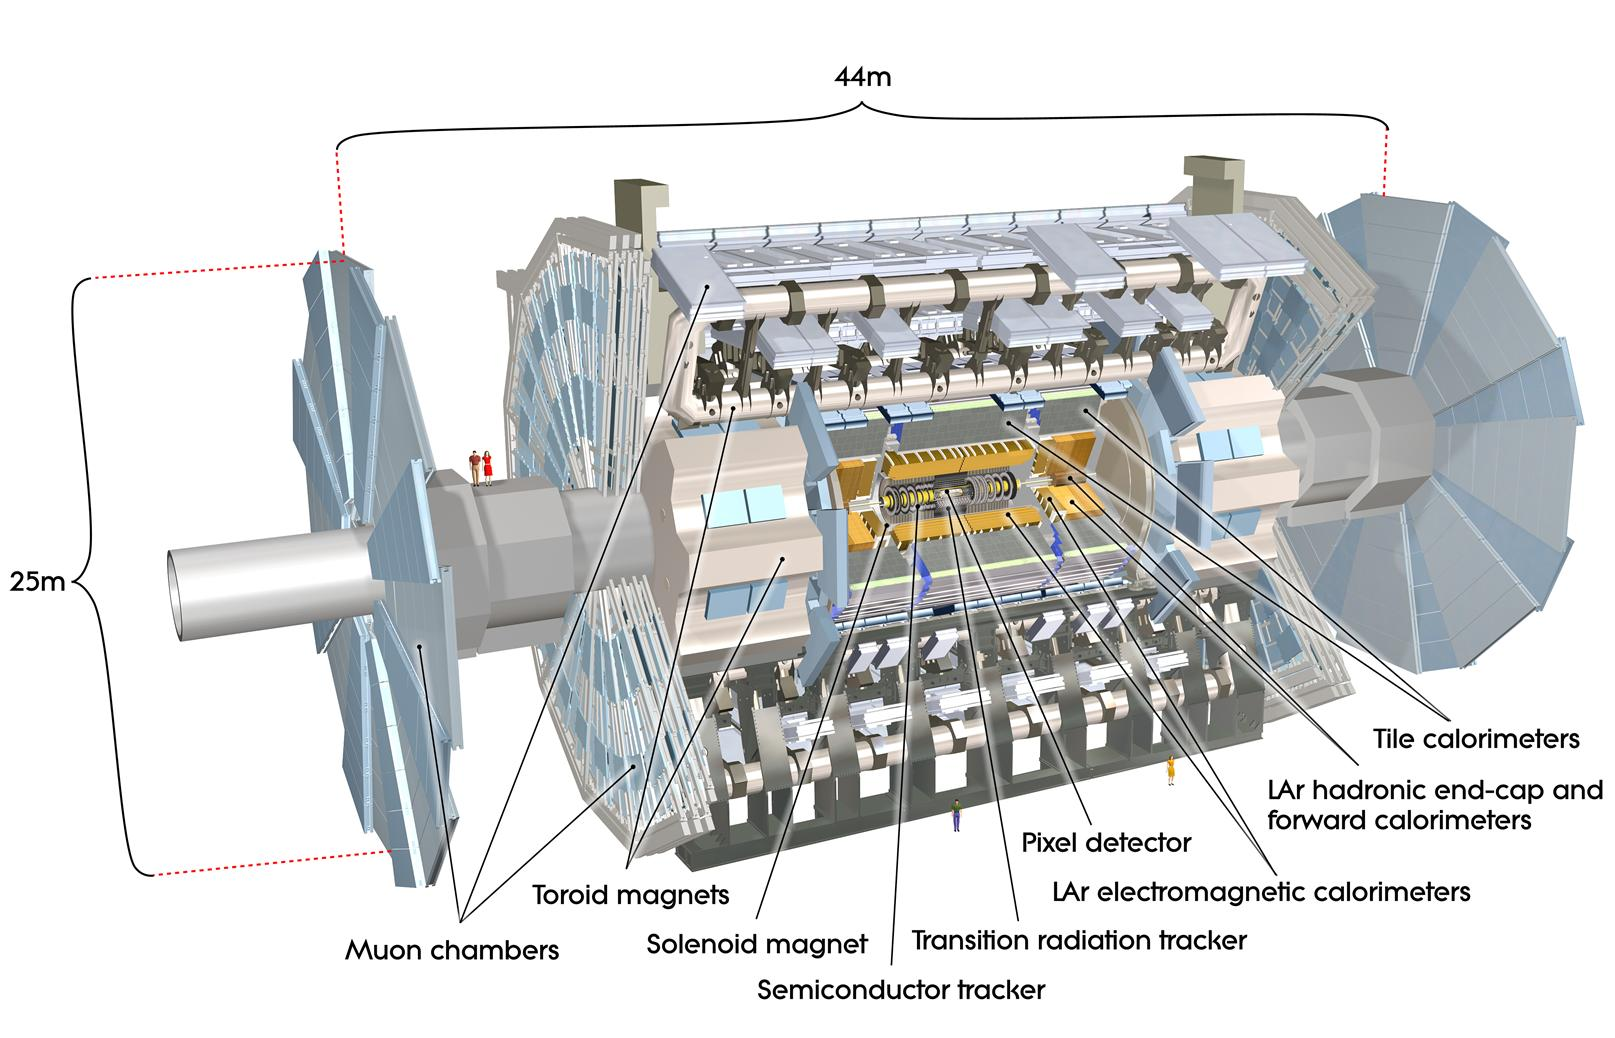
\includegraphics[width=0.75\linewidth]{figures/lhc/ATLASdiagram.eps}
\caption{Cutaway view of the ATLAS detector, with labels of its major components \cite{ATLAS_figure}.}
\label{fig:ATLAS}
\end{figure}

A common coordinate system is used throughout the ATLAS experiment. The interaction point is defined as the origin, with the beam running along the z-axis. Perpindicular to the beam line in the x-y plane is considered the transverse plane, sometimes referred to generally as the transverse direction. Towards the center of the LHC ring is considered the positive x-axis, with up towards the surface of Earth considered the positive y-axis. The azimuthal angle, $\phi$, is measured from the x-axis around the beam. The polar angle is generally written in terms of pseudorapidity, defined as $\eta = -\ln\tan(\theta/2)$, where $\theta$ is the angle from the positive z-axis. The use of $\eta$ is motivated by the fact that differences in $\eta$ are Lorentz invariant. Distances between particles are generally measured as $\Delta R = \sqrt{\Delta\eta^2 + \Delta\phi^2}$.

\subsection{Inner Detector}
\label{sec:innerDetector}

Just surrounding the interaction point is the Inner Detector, designed to track the path of charged particles moving through the detector \cite{IDET-2010-01}. An inner solenoid surrounding the Innder Detector is used to produces a magnetic field of 2 T. This large magnetic field causes the path of charged particles moving through the Inner Detector to bend. Because this magnetic field is uniform and well known, it can be used in conjunction with the curvature of a particles path to measure its charge and momentum.

\begin{figure}[H]
\centering
   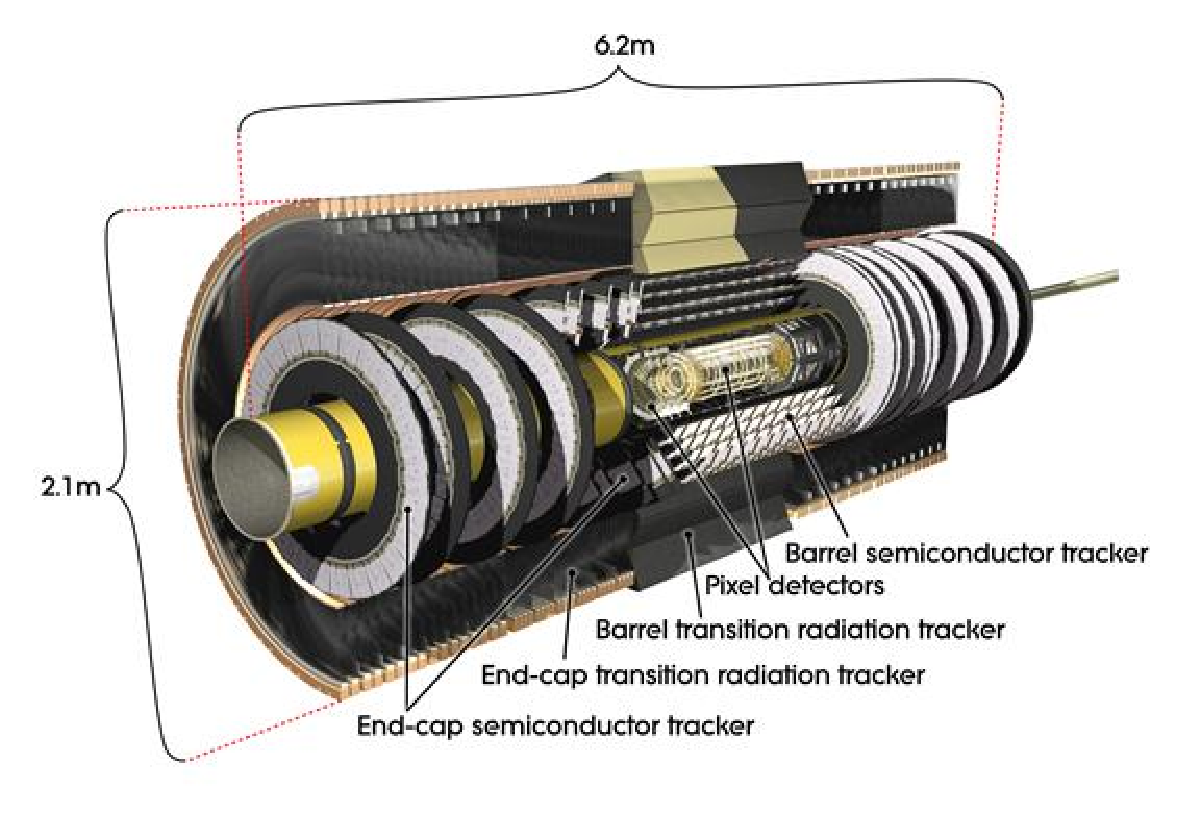
\includegraphics[width=0.75\linewidth]{figures/lhc/InnerDetector.eps}
\caption{Cutaway view of the Inner Detector \cite{caloFig}.}
\label{fig:innerDect}
\end{figure}

The Inner Detector consists of four independent subdetectors - the Insertable B-Layer (IBL), the Pixel Detector, the Semi-Conductor Tracker (SCT), and the Transition Radiation Tracker (TRT). The first three of these detector layers are semiconductor detectors, using silicon as the active material. The last layer, the TRT, uses a gas consisting of Xe, CO$_2$, and O$_2$ as the active material.

The IBL is the innermost of these detectors, beginning just 3.3 cm from the beam axis \cite{larosa2016atlas}. It consists of 224 modules and a total of six million readout pixels. This layer was added in 2014 in order to provide more precise vertex measurements, a crucial aspect of identifying jets originating from $b$-quarks, as described in Section \ref{subsec:bjets}. 

The Pixel Detector is the next innermost layer, and consists of three silicon semiconductor pixel sensors along the barrel, as well as three endcap layers on either side, covering a range of $|\eta|$ < 2.5 \cite{PERF-2012-05}. The Pixel Detector consists of around 80 million pixels, providing a spacial resolution of approximately 10 $\mu m$ in the azimuthal direction and 120 $\mu m$ along the beam-axis. 

The Semiconductor Tracker (SCT) is similar to the Pixel detector, but uses long strips of silicon rather than small pixels to cover a larger spatial area. It includes over 6 million readout strips, allowing the position of charged particles to be measured to an accuracey of 17 $\mu m$ \cite{IDET-2013-01}. Like the pixel detector, the SCT has a pseudo-rapidity range of $|\eta|$ < 2.5. The SCT includes four cylindrical barrel layers and 9 disks in each of the end caps.

The outermost component of the inner detector, the TRT consists of around 300,000 straw tubes filled with ionizable gas, which produces current through a wire in the center of each tube when a charged particle passes through \cite{IDET-2015-01}. Between these staws are layers of material designed to produce transition radiation from ultrarelativistic particles as they pass through each material boundary, amplifying the signal. The position uncertainty in the TRT is higher than the other two, on the order of 200 $\mu m$, but covering a much larger area. 

\subsection{Calorimeters}
\label{sec:calo}

Situated outside the Inner Detector are two concentric calorimeters and a forward calorimeters, designed to measure the energy of particles passing through them. This includes electrons, photons, and hadrons, with muons generally passing through and depositing little of their energy. The full calorimeter system covers a pseudo-rapidity range of up to $|\eta|<4.9$, and is divided into both barrel and end-cap sections.

\begin{figure}[H]
\centering
   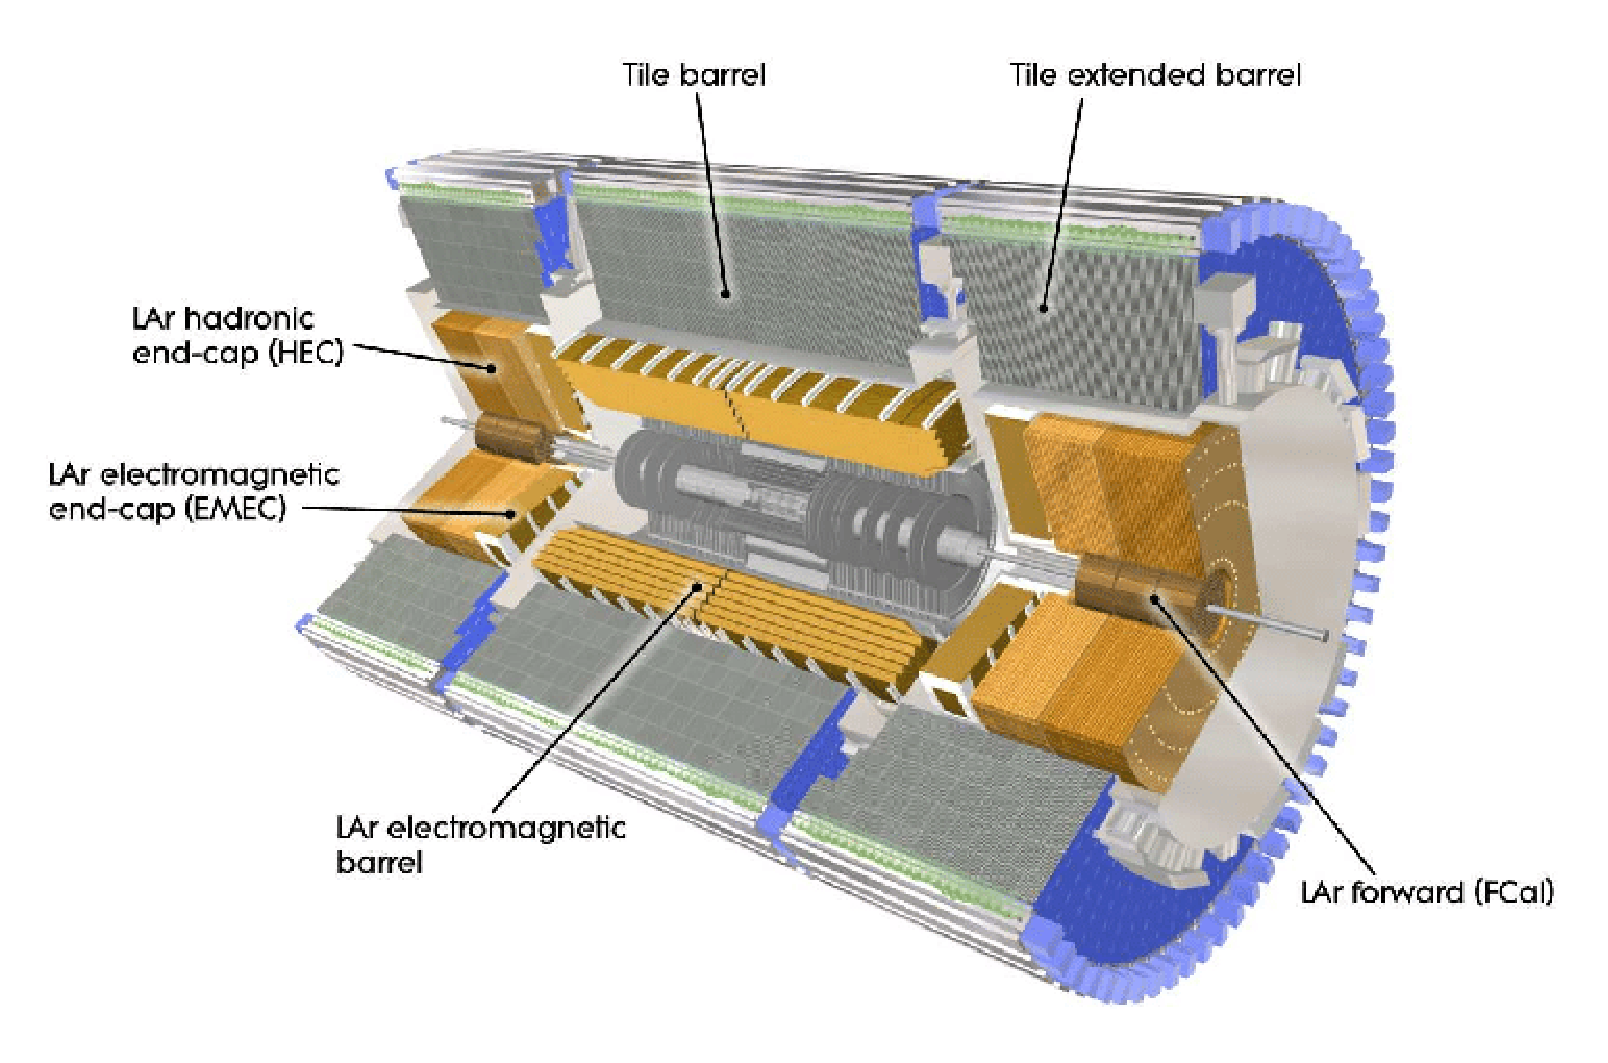
\includegraphics[width=0.9\linewidth]{figures/lhc/calorimeter.eps}
\caption{Cutaway view of the calorimeter system of the ATLAS detector \cite{caloFig}.}
\label{fig:calo}
\end{figure}

The inner calorimeter uses liquid argon (LAr) to measure the  energy of particles that interact electromagnetically, which includes photons and any charged particle \cite{LARG-2009-01}. This calorimeter is also referred to as the electromagnetic calorimeter (EMCal) because, while hadronic objects deposit energy to this calorimeter as well, electrons and photons deposit all of their energy at this stage, and are stopped by this detector, while hadronic objects tend to pass on to the outer calorimeter. 

The LAr calorimeter is made of heavy metals, primarily lead and copper, which causes electromagnetically interacting particles to shower, depositing their energy in the detector. Electromagnetic showers are characterized by their interaction length, $X_0$, the mean distance over which an electron's energy is reduced by 1/$e$. The thickness of the EMCal system varies between 22 and 33 times $X_0$, ensuring electromagnetic showers are well contained by this calorimeter. The showering of the high energy particles that pass through the calorimeter cause the liquid argon to ionize, and the ionized electrons are detected by electronic readouts. 

The EMCal consists of both barrel and end-cap components, with the barrel section covering up to $|\eta|<1.475$, and the end-cap extending from $1.375<|\eta|<3.2$. The LAr calorimeter consists of around 180,000 readout channels, producing a spacial resolution of $\Delta\eta\times\Delta\phi = 0.025\times 0.1$ in the barrel, and $\Delta\eta\times\Delta\phi = 0.025\times 0.025$ in the end-cap. The energy resolution of the EMCal system was tested using an electron test-beam \cite{Aharrouche_2006}, and the energy response was found to be linear within $\pm$0.1\% for electrons with energy between 15 and 180 GeV. 

The outer calorimeter, or hadronic calorimeter (HCal), measures the energy from particles that pass through the EM calorimeter, and is designed to measure the energy of particles that interact via the strong force \cite{TCAL-2010-01}. The strong interaction causes hadronic particles to form hadronic showers, characterized by the nuclear interaction length, $\lambda_{int}$.
The HCal system has an average thickness of around 10 $\lambda_{int}$.
 
HCal also includes barrel and end-cap components. The barrel Tile calorimeter uses steel as the absorber and 500,000 scintillator tiles as the active material, with the signals read out by photomultiplier tubes (PMTs), and covers a range of $|\eta|<1.7$. The hadronic end-cap covers a range of $1.5<|\eta|<3.2$, with copper as the absorber and LAr as the active material. The HCal has a spatial resolution of $\Delta\eta\times\Delta\phi = 0.1\times 0.1$ for $|\eta|<2.5$ and $\Delta\eta\times\Delta\phi = 0.2\times 0.2$ beyond that. Additionally, its energy resolution, measured in test beams, ranges from less than 14\% for pions with $p_T$= 20 GeV to less than 7\% for pions with $p_T>$ 180 GeV \cite{Boumediene:2020cvu}.

Finally, the forward calorimeter (FCal) is built very close to the end pipe, and is designed to absorb forward scattered particles. It covers a range of $3.1<|\eta|<4.9$. FCal has three layers, the first made with copper and the outer two made of tungsten as the absorber, with LAr as the active material throughout. 

\subsection{Muon Spectrometer}
\label{sec:muonSpec}

Because muons are heavier than electrons and photons, and do not interact via the strong force, they generally pass through the other layers of the detector without being stopped by the calorimeters. Their higher mass supresses energy loss through bremsstrahlung radiation, which limits the amount of energy they deposit in the calorimeters. 

The outermost components of the detector are designed specifically to measure the energy and momentum of muons produced in the LHC. The muon spectrometer consists of tracking and triggering systems. The largest of the subdetectors, it extends from the outside of the calormeter system, about a 4.25 m radius from the beam line, to a radius of 11 m \cite{MUON-2010-01}. This large detector system is necessary to accurately measure the momentum of muons, which is essential not only for measurements involving the muons themselves, but also to accurately estimate the missing energy in each event.

 toroidal magnets within the muon system generate a large magnetic field which covers an area 26 m long with a radius from around 5 m out to 10 m. Because the area covered by this magnet system is so large, a uniform magnetic field like the one produced in the Inner Detector is impractical. Instead, the magnetic field that exists in the muon spectrometer ranges between 2 T and 8 T, and is much less uniform. The path of the muons passing through the spectrometer is bent by this field, allowing their charge to be determined. 

1200 tracking chambers are placed in the muon system in order to precisely measure the tracks of muons with high spatial resolution. The path of the muons are tracked by Monitored Drift Tubes, which are drift chambers formed by aluminum tubes and filled with ionizing gas. These tubes produce a multi-layer spatial resolution on the order of 50 $\mu m$.

%\subsection{Forward Detector}
%\label{sec:forwardDet}

\subsection{Trigger System}
\label{sec:trigger}

Because of the high collision rate and large amount of data collected by the various subdetectors, ATLAS produces far more data than can actually be stored. At a bunch crossing rate of 40 MHz, the information from every event cannot practically be stored. Therefore a sophisticated trigger system is employed in real time to determine whether events are sufficiently interesting to be worth storing \cite{PERF-2011-02}. An overview of the ATLAS trigger and data acquisition (TDAQ) system is shown ins Figure \ref{fig:tdaq}.

\begin{figure}[H]
\centering
   \includegraphics[width=0.9\linewidth]{figures/lhc/tdaq.pdf}
\caption{ATLAS Trigger and Data Acquisition system used for Run-2 \ref{AVOLIO20121819}}
\label{fig:tdaq}
\end{figure}

The trigger system in ATLAS involves multiple levels, each of which select out which events move on to the next level of scrutiny. The level-1 trigger (L1) uses hardware information from the calorimeters and muon spectrometer to select events that contain candidates for particles commonly used in analysis, such as energetic leptons and jets. The level-1 trigger reduces the rate of events from 40 MHz to around 100 kHz. The L1 system uses coarse information from the calorimeters and muon chambers to determine whether events will pass onto the next level, and identifies Regions-of-Interest (RoI's) within the detector. 

Events that pass the L1 trigger move to the High-Level Trigger (HLT). This level has access to the full detector data as well as the RoI's identified by the L1 trigger. The HLT takes place outside of the detector in software, and looks for properties such as a large amount of missing transverse energy, well defined leptons, and multiple high energy jets. Events that pass the HLT are stored and used for analysis. Because the specifics of the HLT are determined by software rather than hardware, the thresholds can be changed throughout the run of the detector in response to run conditions such as changes to pilup and luminosity. After the HLT is applied, the event rate is reduced to around 1000 per second, which are recorded for analysis.

The work presented here primarily utilizes the lepton triggers, which are meant to identify events containing leptons passing certain energy thresholds. The HLT looks for leptons in each of the RoI's identified by L1, and performs electron and muon reconstruction as described in Section \ref{obj:ele}, in order to determine whether lepton candidates are present that pass the specified trigger threshold. The specific trigger requirements vary by year, and those used are specified in Section \ref{sec:dataTrigger}.
